\chapter{Appendix list}

\textbf{Appendix Number}
\begin{enumerate}
	\item Interview questions
	\item Transcription: Open discussion with cardiac patients
	\item Field notes: Observation doing rehabilitation program
	\item Transcription: Interview with Vibeke Lynggard
	\item Interview with Hanne Voldgaard Nielsen and Eva Klose Jensen
	\item Economy: Different packages
	\item COPD Project
	\item Exercise equipment used in Herning Municipality
\end{enumerate}



\chapter{Interview questions} \label{interviewquestion}

\textbf{Interview 24/04 2018 med Vibeke Lynggaard, Herning Sygehus} 
\begin{itemize}
	\item Hvad er din rolle og hvordan du er linket til telemedicinsk rehabilitering?
	\item Hvilke generelle processer (målinger, behandlinger, samtaler) kan rykkes hjem til hjemmet og hvilke kan ikke (begrænsninger)?
	\item Hvilke data er relevant at opsamle for hjertepatienter?
	\item Hvilke devices skal tilkobles enheden?
	\item Hvilke træningsplaner er relevante / materiale om eksempelvis ernæring og om sygdommen? 
	\item Er der et specifikt device som vil være oplagt at benytte (telefon, TV)? 
	\item Hvad er din holdning til at erstatte almindelig rehabilitering med tele rehabilitering? 
	\item Vil det være muligt at udføre rehabilitering (træning) i hjemmet via telemedicin?
	\item Tror du man vil opnå samme resultat med den pågældende patient (sygehus vs. hjemmet)?
	\item Kunne det være en kombination eller vil de erstatte 100\%? 
	\item Vil du se tidsmæssige besparelser ved at udføre rehabilitering?
	\item Ser du begrænsninger / ulemper ved at indføre telemedicin i rehabilitering? 
\end{itemize}

\textbf{Interview 15/05 2018 med Hanne Voldgaard Nielsen og Eva Klose Jensen, Sport Center Holing, Herning}


What is the cost of following elements in the cardiac rehabilitation in Herning?
\begin{itemize}
	\item Standard CR
	\item Nurse
	\item Physiotherapist
	\item Dietician 
	\item Education
	\item Technician 
	\item Physical equipment
	\item Brochure
	\item Measurement equipment
	\item IT 
	\item Location
	\item Travel reimbursement
	\item Rehospitalization
	\item Other cost related to hospital after first admission
\end{itemize}

Effectiveness
\begin{itemize}
	\item How do you measure quality of life?
	\item Do you have any measurement in QUALY?
\end{itemize}

\textbf{Interview 17/05 2018 med hjertepatienter, Sport Center Holing, Herning}
\begin{itemize}
	\item Kunne I forestille jer at man flytter rehabilitering hjem i hjemme? 
	\item Kunne man eventuelt flytte noget af rehabiliteringen hjem i hjemmet? Evt. bare undervisningen? 
	\item Ville det være angstprovokerende at åbne op for eget hjem? 
	\item I forhold til det sociale aspekt - vil man savne at mødes to gange i ugen med resten af holdet?
	\item Når i er færdige med det 12 ugers forløb kunne i så forstille jer at i fortsatte med at træne selv eller ville det være nemmere hvis man havde en platform, evt. app hvor trænings programmer samt madprogrammer fra diætist er indskrevet? 
	\item Ville i have problemer med at have en monitor påsat som måler data 24 timer i døgnet? 
\end{itemize}
 
\chapter{Transcription: Open discussion with cardiac patients} \label{open}

\textbf{Interview 17/05 2018 med hjertepatienter, Sport Center Holing, Herning}  

\begin{itemize}
	\item Kunne I forestille jer at man flytter rehabilitering hjem i hjemme?
\end{itemize}
 Nej det kunne jeg ikke forestille mig fordi, jeg tror langt de fleste får ikke gjort det derhjemme, men at man gør noget i fællesskab fremfor at gøre det selv så er der mange som ikke går det gjort. 

Enighed blandt af patienter. 

Bruger man det ikke allerede nu eller er det forsøgsbasis? Har set noget om det i TV får man brugte telemedicin hos KOL patienter. 

En anden ting er sikkerheden i at komme herud fordi der er en sygeplejerske og en fysioterapeut så de kan helt principielt samle en op hvis man falder af cyklen. Det vil de ikke kunne hvis man sidder derhjemme. Der vil gå flere minutter inden der kommer hjælp. 

Man hører tit at nu skal vi til at gøre noget ved vores krop og køber en motion cykel hjem til. Den motionscykel får man brugt tre gange og så bliver den stillet væk igen og det er fordi man gør det alene, jeg tror det er derfor. 

\begin{itemize}
	\item Kunne man eventuelt flytte noget af rehabiliteringen hjem i hjemmet? Evt. bare undervisningen? Ville det være angstprovokerende at åbne op for eget hjem? 
\end{itemize}
Nej det tror jeg ikke. Så tror jeg de forskellige ville gøre mere ud af det. 

Hvordan skulle man rent praksis gøre det i hjemmet i forhold til trænings udstyr? 
Line: man skal sætte cykel ud til borger eller også skal træningen i hjemmet være baseret på øvelser som ikke kræver udstyr. Matilde: Det man har gjort med KOL projektet er at man får en KOL kuffert hvori man har det udstyr der skal bruges. 

\begin{itemize}
	\item I forhold til det sociale aspekt Vil man savne at mødes to gange i ugen med resten af holdet?
\end{itemize}

Ja det ville man, jeg tror det bliver det største problem. Det bliver for upersonligt, man vil komme til at savne at få en snak om alt muligt andet end lige sygdommen. 

Jeg kan sammenligne det med en vandregruppen som jeg er med i hver tirsdag. Om det stormer, regner eller sner kommer vi altid afsted. Hvis jeg ikke var med i sådan en klub havde man ventet til vejret var bedre. Så tror jeg også at hvis man skal træne hjemme har man ikke lyst og udsætter det til i morgen. 

Her på holdet er man mere eller mindre tvangs indlagt. Der skal være en god til at melde pas. 

\begin{itemize}
	\item Når i er færdige med det 12 ugers forløb kunne i så forstille jer at i fortsatte med at træne selv eller ville det være nemmere hvis man havde en platform, evt. app hvor trænings programmer samt madprogrammer fra diætist er indskrevet
\end{itemize}
Det ville helt klart være en opstrammer til at man fortsætter. Herning kommune har nogle trænings timer for osteporose patienter hvor jeg har været med de sidste par år. Det er en gang om ugen i et fitnesscenter, det er rigtig godt. Regner med at skulle fortsætte der når jeg er færdig her. Det er der ikke nogen tvivl om for der har vi også et godt sammenhold. Det trækker når der er andre. Det betyder meget at det ikke bare er træning men også det sociale. Vi mødes i god tid og snakker også lidt bagefter. 

Eksempel fra Canada: målinger bliver foretaget i hjemmet og sendt direkte til egen læge og sygehus som opdatere 24 timer i døgnet. Hvis man bliver forværret sender de en ambulance og kører ham på sygehuset. Mange folk bliver redet på den måde. 

Tidligere blev det nævnt at nogle borgere måler blodtryk. Hvis der er nogle svingninger i de målinger ville det opdages i tide og man kan på den måde fange patienten inden de blive forværret alvorligt. 

\begin{itemize}
	\item Ville i have problemer med at have en monitor påsat som måler data 24 timer i døgnet?
\end{itemize} 
Nej det ville jeg ikke have et problem med. Man ville blive positivt overvåget. Det ville give en tryghed hvis man var bange. 

Jeg har for år tilbage haft en døgnmåler på. De er nok blive mindre nu end de var for 10 år siden. Det er 12-15 år siden jeg har haft det. 

Jeg havde og sådan en og kan godt huske den nattesøvn jeg fik. Man sov næsten ikke. Den strammer jo op hver halve time, men det var heldigvis bare et døgn. 


\chapter{Field notes: Observation doing rehabilitation program} \label{field}

Observationer under træning: 
\begin{itemize}
	\item Vil gerne bibeholde 12 ugers forløb da det er her man lærer øvelserne
	\item Ville være optimalt at indsætte som forløb efterfølgende – gavnligt hvis man kunne tjekke op / sikre sig at borgeren har trænet (”det er selvfølgelig for min egen skyld, vi er voksne mennesker så brude bare hanke op i sig selv”) 
	\item Ses af efter 3 år er borger tilbage på samme stadie fordi de ikke følger op på træningen 
	\item Bliver også tilbudt borgere som ikke er ramt er hjertesygdom men er i risiko for at udvikle hjertesygdom 
	\item 8 borgere til første træning
\end{itemize}

Observationer under undervisning:
\begin{itemize}
	\item Undervisning i risikofaktorer 
	\item 13 deltagere til undervisning
	\item Afsluttende cykel test, samtale og afsluttende kontrol i hjerteklinikken (1-2) uger efter træning. Tjekker kolestol, blodtryk og andre målinger – kan tilrette medicin herefter 
\end{itemize}




\chapter{Transcription: Interview with Vibeke Lynggard} \label{vibeke}



\textbf{Interview 24/04 2018 med Vibeke Lynggaard, Herning Sygehus}

\begin{itemize}
	\item Hvad er din rolle og hvordan er du linket til telemedicinsk rehabilitering? 
\end{itemize} 
Jeg arbejder som projekt sygeplejerske, men er lige blevet færdig med ph.d., så er lidt in between positions. Når man er på hjerteafdeling får man ekg’er som er blevet taget i ambulancen. Dem får man ind og skal se på en skærm, det er så primært den læge som tager imod i forhold til om patienten skal til en direkte ballon udvidelse eller skal ind omkring Herning sygehus først eller kører patienten til Århus. Telemedicin i det man går ind og kigger på en skærm. 

\begin{itemize}
	\item Er du linket til patienternes rehabilitering efter indlæggelse? 
\end{itemize} 
Ja, men det er projekter som patienter kan vælge at deltage i. Det har ikke noget med rehabilitering at gøre. Men vi kommer alligevel til at lave rehabiliterende tiltag. Mit arbejde går ud på at vi har projekter med medicinalindustrien og så har vi patienter inde som afprøver ny medicin. Så kommer de til os en gang i måneden i muligvis 5 år. I og med vi er projekt sygeplejersker så kommer man til at lave rehabiliterende tiltag i form af vejledning og pleje af en måske mulig stress tilstand. 

\begin{itemize}
	\item Hvilken rehabilitering udfører man for patienter i dag? 
\end{itemize} 
Det er pr. 1/1 2017 blevet lagt ud til kommunerne i stedet for regionerne, så det er ikke herinde på hospitalerne længere. Der kører dog et hold kontinuerligt med 12 patienter med de sværest syge, dem der har problemer med pumpefunktioner af hjertet og nogle hvor man ikke kunne åbne alle kransåre. Det er altså de dårligste patienter som bliver rehabiliteret på hospitalerne. Eller er det lagt ud i kommunerne og har været der det sidste 1,5 år hvor de træner patienterne i 12 uger 2 gange i ugen og bliver undervist en gang om ugen i et ønske om at lægge det ud der hvor borgeren er geografisk. Eks regions Vestjylland er meget spredt. 

\begin{itemize}
	\item Hvad gennemgår de 12 patienter, som kommer ind på sygehuset til rehabilitering? 
\end{itemize} 
De får lavet en maksimal symptom betinget stress test på en kondicykel hvor man beder dem cykle så meget de kan. Her øger man loads i watt. Så har man et udgangspunkt, efter de 12 uger laver man testen igen og ser om de har forbedret sig. Fysioterapeuten har et program – dette gælder på samme vis i kommunerne. De laver både cardio stress for at få pulsen op og så laver de muskel streching. Der er nogle nationale retningslinjer for hvor meget intensitet man skal træne med og hvor mange reppitionerne man skal lave. Der er både dem som har blodpropper i hjertet, dem som har nedsat pumpefunktion, dem som har fået en ny hjerteklap og dem som har fået en pacemaker. De har meget forskellige behov og skal derfor træne forskelligt. 

\begin{itemize}
	\item Hvilke målinger bliver der lavet?
\end{itemize} 
Man måler vægt, højde og taljemål, blodtryk og puls. Det er lovpligtigt at patienten skal igennem dette forløb, så det er noget man skal sætte ind efter. Kunne være muligt at sætte telemedicinsk forløb ind efter de 12 uger – de 12 uger er fase 2 rehabilitering. Patienter skal tilbydes fase 3 men rigtig mange vælger det fra fordi de skal tilbage på arbejdsmarkedet. Rigtig mange stopper med vanlig care og der er et kæmpe frafald i at fastholde sunde livstilsvaner. Her kunne det virkelig være relevant at indføre. Passe på med at tænke de ind som erstatning for de 12 ugers forløb da det er lovpligtigt og meget evidens baseret. Det er på klasse 1 recomentaion fra de amerikanske og europiske hjerte institut, så det er ikke noget man bare erstatter. Fase 3 handler om at fortsætte og vedligeholde gode motions- og kostvaner, fastholde et rygestop. Screener også patienter for depression. De udfylder et spørgeskema som hedder HADS – hospital and society depression score. Det vel også en form man kan udfylde i hjemmet. Der ligger en algoritme bag og så kommer der en score ud. Den kan sige om man skal kontakte egen læge. 

\begin{itemize}
	\item Er der nogle af målingerne som kan tages i hjemmet i stedet for på sygehuset?
\end{itemize} 
Det er svært at lave et taljemål selv, da det i forvejen er et meget usikkert mål. Det plejer derfor at skulle være en sundhedsplejerske som tager dette. Der er også meget bias hvis patienten selv skal måle taljen. Så forsvinder objektiviteten. Spørgeskema kunne derimod sagtens tages i hjemmet. Blodtryk kunne også. Ved ekg får man kun tre afledninger hvis det måles i hjemmet. Ved ekg vil man gerne se om der er tegn på iltmangel og det kan man ikke ret godt på tre afledninger, der skal man helst have 12 afledninger. Hvis der var en form for en censor eller så man husker at tage sin medicin – man skal trykke på en knap når man har taget sin medicin eller kommer der en advarsel. Der findes også scoringstest hvis man tobaks ryger hvormed man kan se hvor nikotin afhængig man er. Der kommer også en score fra algoritme som siger om det er plaster eller tyggegummi. 

\begin{itemize}
	\item Hjertesygdomme er ofte afledt af livsstil sygdomme. Er rehabilitering ligeså meget at man skal af med sine dårlige vaner? 
\end{itemize} 
Hjerterehabilitering består exercise, education og social, at man også forholder sig deres sociale. Der er altså trepinde og der er meget stærk evidens for at det virker. Så det ene kan ikke stå alene. En hjertepatient bliver pludselig syg og exercise er derfor vigtig, men det går meget på at få pulsen op og lære dem nogle sunde motionsvaner. Motion fylder derfor ligeså meget som uddannelse og risikofaktorer. 

\begin{itemize}
	\item Hvilke data er relevant er opsamle i hjemmet – skal der sætte devises til? 
\end{itemize} 
Rehabilitering går meget på at man kan tracke at de overholde deres sunde livsstil og adfærd. For en patient med hjertesvigt kunne man benytte en vægt. Hvis man via tablet kunne interagere med sundhedsfaglig ville dette være meget relevant. Herved kunne genindlæggelser undgåes. Puls, blodtryk og iltmætning er ikke det som er vigtig i rehabilitering af en hjertepatient. Det er vigtigt at patienten lærer at mestre livet og komme tilbage til livet og arbejdsmarkedet. Den gennemsnitlige hjertepatient er omkring 60 år så det er ikke de ældre ældre. Depression score screeninger en gang i måneden kunne godt være en anbefaling, herved kan patienten fanges før de ryger ud i en depression. Det tricker en handling. Det er et spørgeskema som også høre ind under de nationale kliniske retningslinjer. Nogle patienter er meget deprimeret og det opdages for sent fordi de kun tilses på sygehus hver tredje måned. Hvis kufferten fortæller at spørgeskemaet ikke er udfyldt og det skal gøres i morgen, så der kommer en påmindelse. Mange af dem som har haft blodpropper i hjertet er i risiko for at udvikle en depression. Spørgeskema udfyldes 6 uger efter udskrivelse. Så det er en engangsting som både laves i kommuner og hospital afhængig af hvor de træner henne. I de 12 ugers forløb er der både fysioterapeut og sygeplejerske tilstede og så kører de et forløb som hedder læring og mestring hvor der også er en tidligere patient med som medundeviser ud fra den tanke at de selv har levet med en hjertesygdom. Så formidler man erfaringsviden sammenmed professionel viden. Man skal være meget opmærksom på lovgivning hvis det skal erstatte fase 2. 

\begin{itemize}
	\item Hvad er vigtig i forhold til ernæring hos hjertepatienter? 
\end{itemize} 
Hjertepatienter bliver tilbudt forløb hos diætist. Det har man valgt i region Midtjylland. Ernæringsenheden ligger i Holstebro. Det er ikke alle som møder op. Der er oplæg en dag og nogle praktiske øvelse, det er ofte 2 dage man er afsted. Det ville være oplagt at ligge madplaner ind på appen. Og også systemer hvor man på en eller anden måde kan logge en kostdagbog. Sådan nogle ting virker godt for nogle for andre kan det være en belastning. Denne type apps findes allerede og man kunne så linke til tv køkken hvor nogle kokke laver det. 

\begin{itemize}
	\item Er der nogle platforme / devises der vil være oplagt til telemedicin? 
\end{itemize} 
Tablet og telefon ville være oplagt til telemedicin. Jævnfør alder, de er forholdsvis ungdommelige og ville godt kunne håndtere en tablet. 

\begin{itemize}
	\item Hvad er din holdning til at erstatte almindelig rehabilitering med telerehabilitering? 
\end{itemize} 
Det kunne sættes i stedet fase 3. Hvis der er evidens for det kunne man så forkorte de 12 uger hvormed de sidste 6 foretaget i hjemme ved telemedicin? Fællesskab med de andre på holdet tabes lidt, hvis der er god dynamik på holdet fungerer det rigtig godt. Der er lavet kvalitativ interview hvor det ses at det vægtige er de andre patienter, den erfarende patient. Det skal derfor afdækkes. Det skal testes op imod hinanden. Vil også give etiske udfordringer, det plejer man at holde på fire niveauer. Man må ikke give patienten noget der måske kunne være dårligere, når vi ved at dette er det bedste kan det ikke tages væk. Kunne godt følge tanken, da det for mange på arbejdsmarkedet er nemmere at tænde for tablet og koble sig på holdet om aftenen. De fleste kommuner har både formiddags og eftermiddagshold, rigtig mange kan blive godt gjort af arbejdsgiver, så mange er ikke på fuldtid fordi det er en del af behandlingen. Så de dage de træner har de fri til det. Fase 3 kunne sagtens være en god ide. 20\% gennemføre ikke fase 2 og det er kun 50\% som møder op til fase 2, så allerede her er det en ret stor gruppe. De patienter som ikke møder op til fase 2 har formentlig en hel del konkurrende sygdomme fordi der er nogle kendte barriere. Kvinder har tindens til ikke at møde op og det er fordi når de bliver hjertesyge er de ofte lidt ældre og har ofte konkurrende sygsomme. Derudover kan der være geografi og noget med at køre. Bare hvis man skal køre 15min kan det være svært for nogle. I sådanne situationer kunne det være en mulighed for at tage med hjem, men vil aldrig supportere at de springer fra. Det her er det tilbud som vi ved der virker og hvis det eksempelvis er en som har KOL samtidig er man meget udfordret. Træner er altid meget individualiseret. Man ved også at lav sosu økonomisk status er en barriere til at møde op så der kunne også være noget. Helt sikkert, der er et kæmpe behov. Især hvis alternativet er at de ikke får noget. Dog hvis det er vildt dyrt har vi igen en skævhed i hvem er det som vælger det til – hvis det er en app som koster penge. Det er et kæmpe område. Kunne også være dem som er henvist men ikke dukker op, men hvem skal finde dem? Det er den sygdom med størst dødelighed og lige nu lever 300.000 mennesker med sygdommen i Danmark. Prævalensen er stigende fordi vi bliver bedre og bedre til at behandle selvom mortalitet er faldende. Egentlig også incidensen fordi man bliver bedre til at spise sundere og så videre. Den er svagt faldende eller stabiliserende, men selv prævalens (forekomsten) er stigende.

\begin{itemize}
	\item Skal det være en kombination eller erstatte den almindelig rehabilitering?
\end{itemize}  
Dem vi ikke når ville det her være et bedre tilbud end ingenting hvis telemedicin handler om at man kan koble sig på forskellige trænings sessioner, koble sig på forskellige undervisning og viden om mad. Det der er evidens for er at det andet som virker. Det er internationalt anerkendt. Kan godt se muligheder. 

\begin{itemize}
	\item Vil du kunne se tidsmæssige besparelser ved at indføre telemedicinsk rehabilitering?
\end{itemize} 
Ja bestemt, da patienten ikke skal fragte sig og selvfølgelig også for sundhedspersonale. Og hvis det er ligeså godt til at forhindre genindlæggelser som man ved hjerterehabilitering er så er det også sundhedsøkonomisk. 

\begin{itemize}
	\item Hvilke begrænsninger og ulemper ser du ved at indføre telemedicin i rehabilitering? 
\end{itemize} 
Jeg ser ingen begrænsninger. Hvis man tænker at de her sker efter vil der ikke ses nogle begrænsninger. Hvis det ses som en erstatning er der selvfølgelig det sociale da patenter hygger sig, drikker kaffe, snakker med hinanden. Men det er aldrig vist i projekter at det er det som der som sådan har en betydning for genindlæggelser. Men som sagt hvis du spørger patienterne selv vil de sige det har en stor betydning, men det er svært at skære alle over en kam fordi nogle vil mene det er rart ikke at skulle forholde sig til andre. Måske skal man screene patienter så man finder det rette, dette kan gøres ud fra læringsstile, ud fra risiko behov. 

\chapter{Interview with Hanne Voldgaard Nielsen and Eva Klose Jensen}
\textbf{Interview 15/05 2018 med Hanne Voldgaard Nielsen og Eva Klose Jensen, Sport Center Holing, Herning}

Risiko: nogle der bliver dårlige og akut hjertestop – risiko i af være i hjemme og kan derfor ikke få som hjælp hvis man er derhjemme. 

Primært de patienter som bor længere væk fra kommunen takker nej til tilbuddet fordi der er for langt til behandlings stedet. Dette ses ikke i Herning kommunen. Yderområder er flest af dem som takker nej til kommunerne. De 10\% dårligste skal blive på sygehusene for at få træning. De fleste som bor tæt på kommunen tager imod tilbuddet. 

Grunde til at takke nej: Depression ikke magtede det, syg ægtefælde, dement. Stoppet undervejs – dårligt knæ. 

200 om året hvor kun 5 har sagt nej. Mail sendt. 

Hjerterehabilitering har fået penge af kommunen. 
Det som koster mest er lønninger. 
Sygeplejersker timer køber de fra regionen: 2*21 timer, 48 uger om året. Lidt dyrere fordi de får løntillæg. Ca. 308 kr. i timen – pga. tillæg fordi de kommer fra hjerteafdelingen. 
To fysioterapeuter: 26 og 28 timer om ugen, 48 uger om året (130.000 pr. kvartal i fys timer). Omkring 600.000 om året (pensionstillæg osv. Indgår). Erfarne og på højere løntrin, får derfor højere løn. 
Derudover diætist: fire gange om året af 3 timer + forberedelse (2 timer) ca. 20 timer om året.  
Altid fire hold i gang. Cirka 200 patienter om året. 
Rygestop vejleder: tilbyder til alle borger som har brug for det. Udfordring til hjertepatienter er at de ikke kan overskue rygestop og træning på samme tid - en ting af gangen. Kunne tage det efterfølgende og vil fortsat være betalt af kommunen. 
Løsningen er ikke den billigste. 

1 gang om ugen med undervisning, kost, livsstil, motion, sygt og rask hjerte, psykisk, fremtid, leve med sygdom. Først afklarende samtale og test - træning - slutter af med test. Sygeplejerske har alt samtale med hjerteklinikken og følger op på medicin.   

Engangsinvestering – havde ikke et sundhedscenter og skulle derfor købe det hele fra nyt. 280.413 kr. undervisning materiale, kontormiljø, sikkerhedsudstyr, roll ups, test cykel (76750), blodtryksmåler  - implementeringsprisen. Sendt på mail.  

Bestiller materiale gennem hjerteforeningen som de får udleveret. Patienter får en bog fra hjerteforeningen hvor mange informationer.

Ikke noget separat kommunikation system – foregår på mail, e-boks osv. 

140.000 om året for leje af lokale (dette må ikke blive publiceret) 

Rejseudgifter: hvis de har over 50 km eller er ude af stand til at rejse – men ingen udgifter hertil. 

HjertekomMidt database – database til alle kommuner i region Midtjylland som man skal oprettes i. 

Udgifter til kurser og uddannelse – 10.000 om året. 
Læringsmestring konceptet, erfarings deling hvor tidligere patient deltager. Deres historier og erfaringer gør patienter i stor grad brug af. 


\chapter{Economy: Different packages} \label{economics}

\begin{figure}[H]
\centering
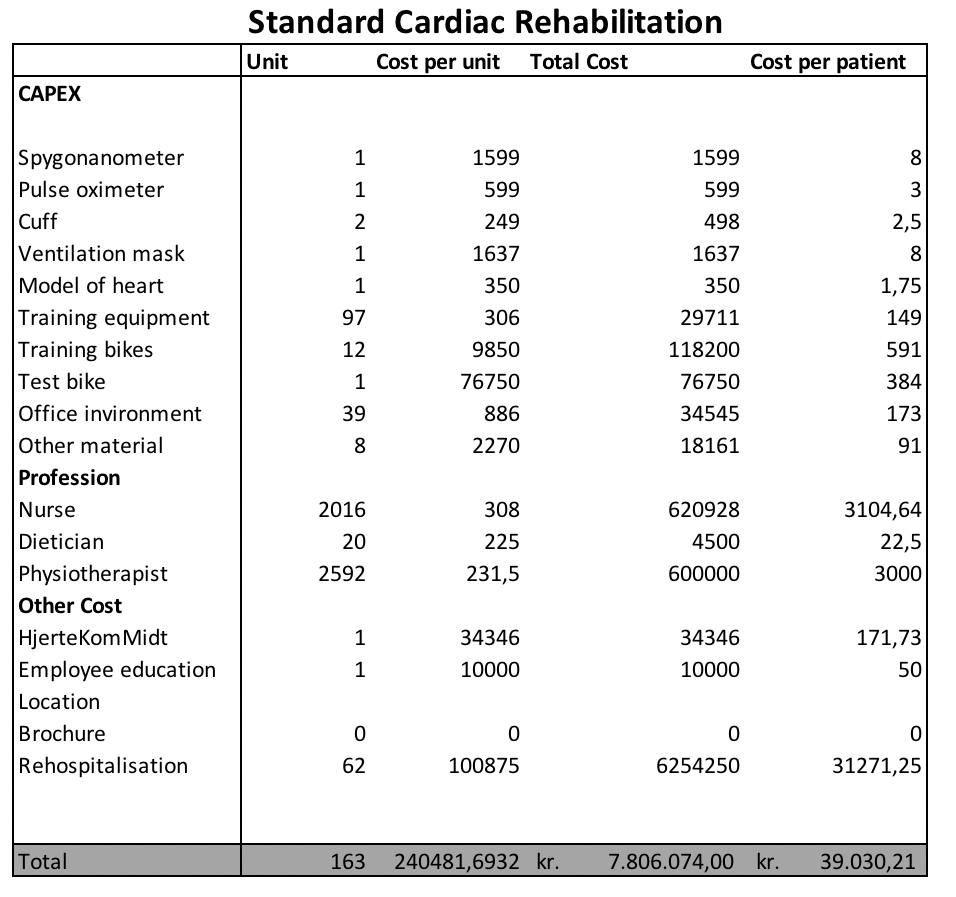
\includegraphics[width=1\textwidth]{Figure/SCR.png}
\caption{??}
\label{fig: SCR}
\end{figure} 
\begin{figure}[H]
\centering
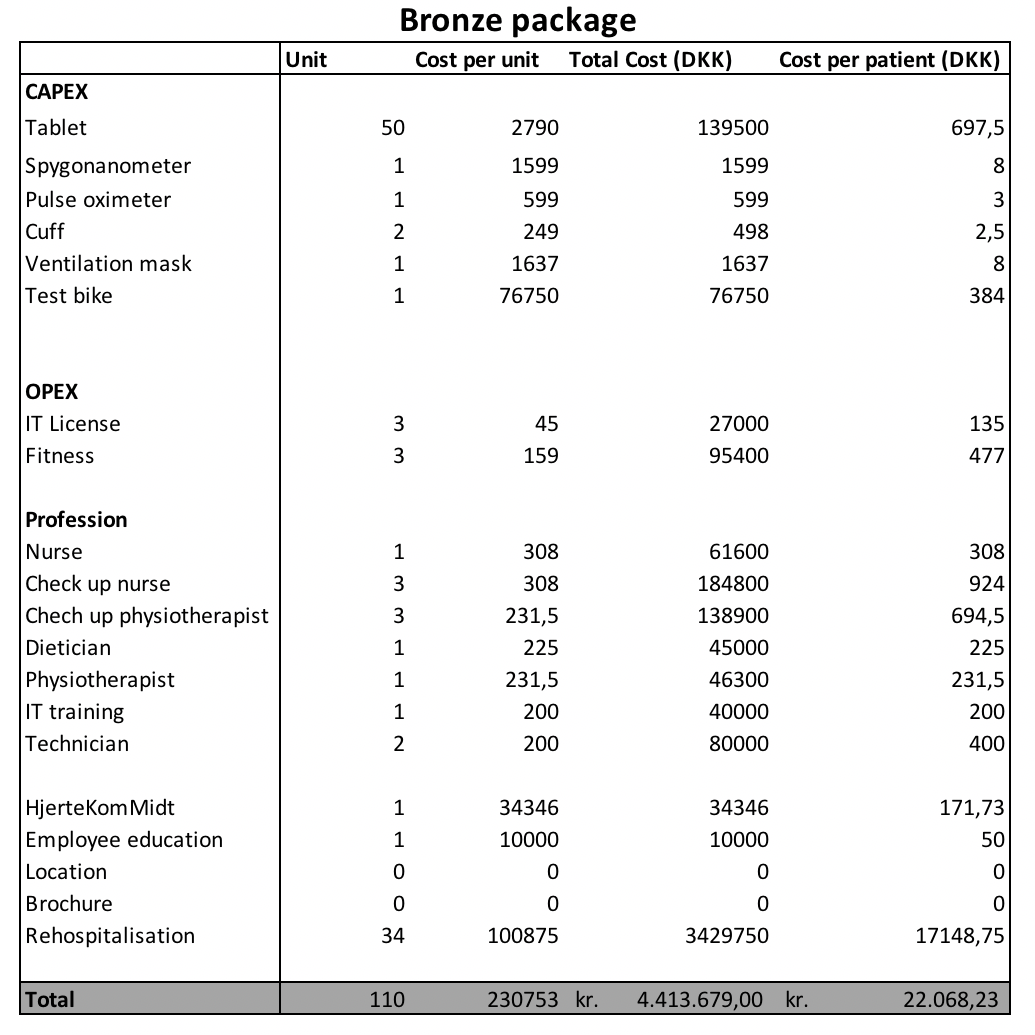
\includegraphics[width=1\textwidth]{Figure/Bronze.png}
\caption{??}
\label{fig: Bronze}
\end{figure} 

\begin{figure}[H]
\centering
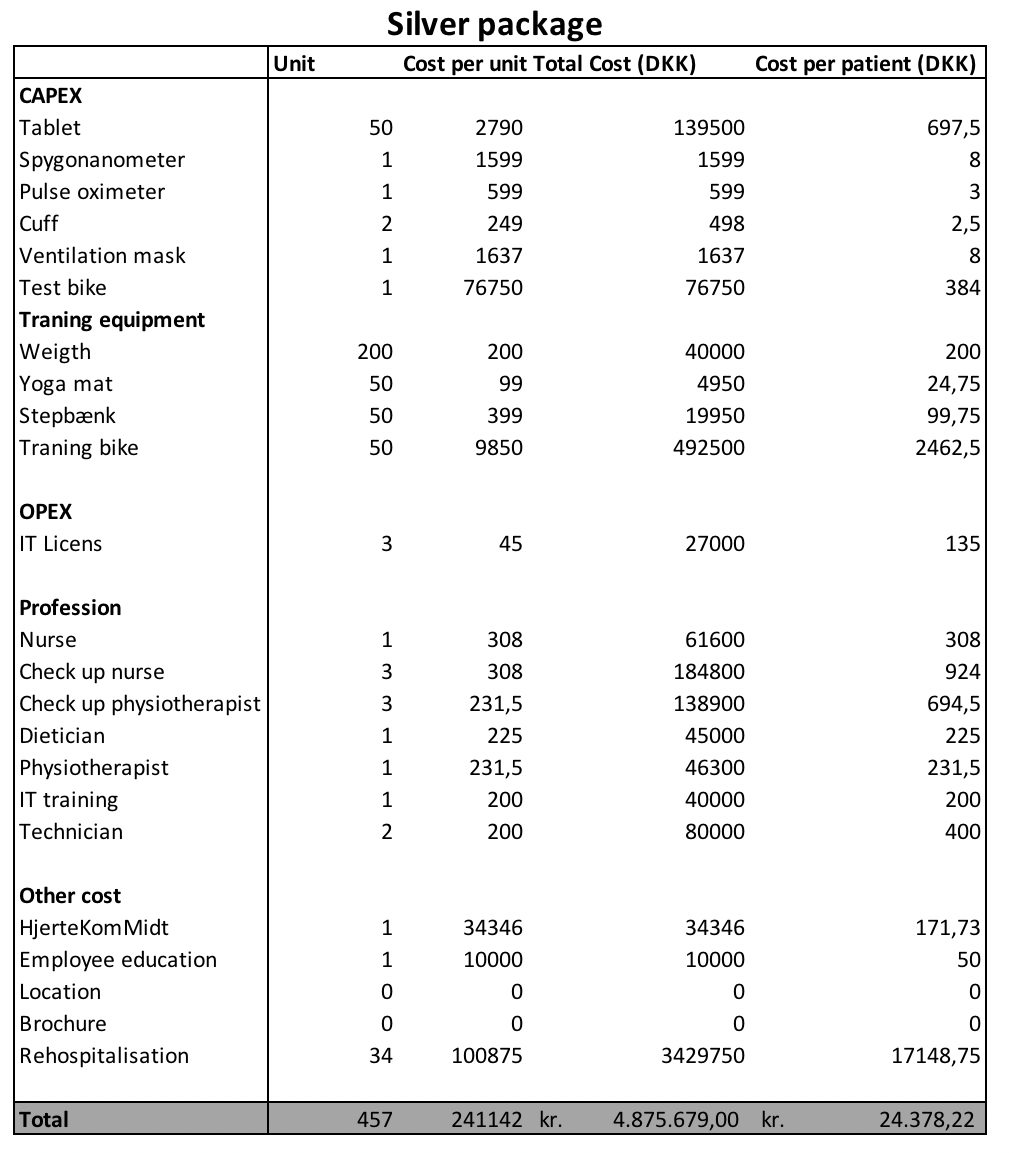
\includegraphics[width=1\textwidth]{Figure/Silver.png}
\caption{??}
\label{fig: Silver}
\end{figure} 

\begin{figure}[H]
\centering
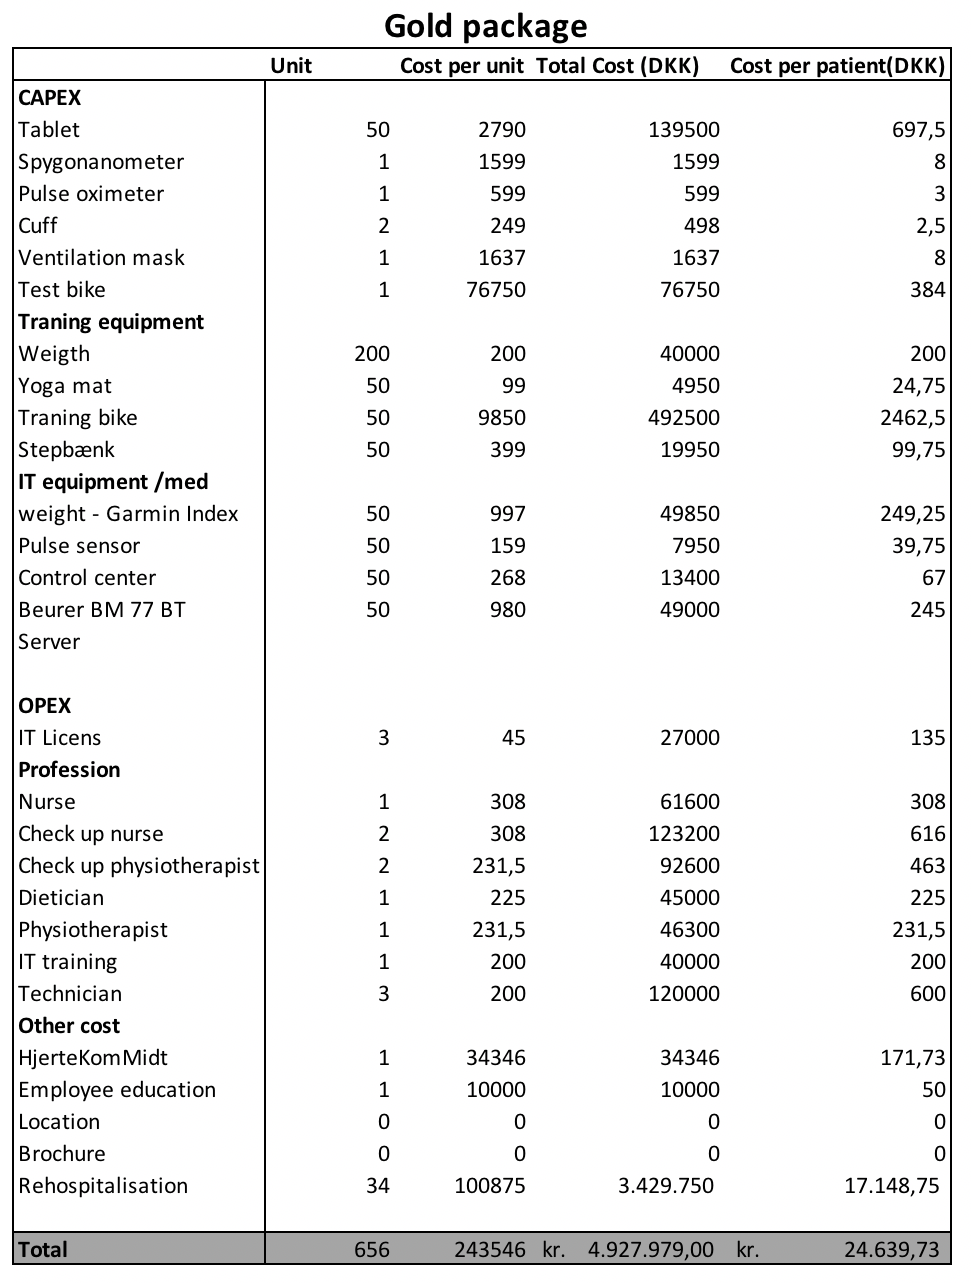
\includegraphics[width=1\textwidth]{Figure/Gold.png}
\caption{??}
\label{fig: Gold}
\end{figure} 


\chapter{COPD Project}
\textbf{Interview 23/05 2016 med Borgere fra Skanderborg Kommune}

\begin{itemize}
	\item Evidens og indledning
\end{itemize}
Patientafsnittet for Skanderborg løsningen er primært baseret på interviews med borgere og en fysioterapeut, som arbejder med løsningen. Dertil er der dog også brugt en smule evidensbaseret artikler af lavere kvalitet (bl.a. fordi de ikke er randiomiserede og der var få forsøgspersoner). Artikler er også udenlandske, hvilket også har betydet, at det har været nødvendig at overveje om det kan overføres til Danmark. Afsnittet er bygget op omkring en samtale med to borgere over Skanderborg løsningen efter de havde trænet. Senariet, som var blevet sat op var 8:8 – alle kunne høre og se hinanden.

Patientafsnittet for digital monitorering er primært baseret på videnskabelige artikler. Artiklerne er af svingende kvalitet i forhold til, hvor mange forsøgspersoner der er, og hvor evidensbaseret de er. Flere af artiklerne er desuden ikke randiomiserede, mangler kontrolgrupper og er bygget på andre artikler, hvor opbygning af studiet er ukendt. Disse ting gør, at deres indhold til kan tages som den altafgørende sandhed, men på grund af kvantiteten af artikler, som siger det samme, bruges de forskellige dele, som de har tilfreds samt patientudtalelser.

\begin{itemize}
	\item Etiske forhold
\end{itemize}
Når man kikker på de etiske forhold, det vigtigt at kikke på det ud fra idealer, konsekvenser og pligter i forhold til det etiske hjul (Henvis til tidligere). Dette er blevet gjort ved at kikke på nogle af de overvejende ud fra samtale med borger, som bruger løsningen og egne overvejelser i forhold til løsningen. Efter samtale med borgere blev det gjort klart, at de ikke selv har overvejet nogle etiske problemstillinger ved løsningen. De så det f.eks. ikke som grænseoverskridende at åbne deres hjem over skærmen. En borger udtalte at løsningen ”absolut ikke er grænseoverskridende. Jeg har ikke noget at skjule.”. Så borgeren så det ikke som et overgreb. Dog er det vigtig at påpege, at det er individuelt, hvordan man har det med det, og bør være med i tankerne, når det skal implementeres ved andre. Derudover kan løsningen også komme til at virke stigmatiserende og forstyrrende i hjemmet for borgeren. Udtalelse fra Mette Hammer, fysioterapeut ”Jeg har haft en borger, som synes, at fjernsynet virkede stor og var grimt, så hun dækkede det til med en dug.”. Så særligt konsekvenser individuelle og skal overvejes ved implementering af denne teknologi. Teknologien: lyden ved den ene deltager hakker en del, Mettes billeder hakker, kommer i ryk når hun bevæger sig og fryser af og til. Mette siger at der har været problemer med Kurts lyd gennem træningen.

\begin{itemize}
	\item Kommunikative forhold
\end{itemize}
Patient
-	Hvordan oplever du telemedicinsk træning i forhold til traditionel træning?
Svar:
Robert: Synes det er godt og virker rigtig fint. Fri for at skulle ud og køre. Fruen har bilen, derfor skulle han have en taxi hvis han skulle nogle steder hen. Går lige så meget op i det som hvis han skulle til traditionel træning. Kurt: rigtig godt, slipper for at komme ud i regnvejr. Kan gøre det når det passer. Dårlig forbindelse ind i mellem ellers er det ikke så sjovt.

-	Kan du se ulemper ved den telemedicinske træningsform?
Svar:
Kurt: hvis forbindelsen er i orden, er der ingen ulemper. Billede og lyd skal være i orden. Lyden er særligt et problem. Når man ikke kan høre noget, kan man ikke være ordentlig med. Robert: vigtig at billede og lyd er i orden. Roberts går godt igennem. Generelt: billedet er godt ved begge, men lyden er dårlig ved Kurt. Robert prøver at hjælpe Kurt.

-	Ville du hellere træne på et center frem for telemedicinsk træning?
Svar:
Robert: Ville hellere være til træning med nogle personer i stedet for over fjernsynet. Oplever ikke det sociale samvær på samme måde. En god løsning men en nødløsning. Ikke socialt på samme måde som når man er tilstede (sammenligner det med en kæreste). Programmet kører rigtig godt og Mette er god til at illustrer og rette på dem – et rigtig godt alternativ.

-	Kan du mærke, at det hjælper at træne? Får du mere overskud og hvis ja, hvordan
kan det mærkes?
Svar:
Robert: Hjælper bestemt, kan mærke det i musklerne når man udfører øvelserne så godt som man kan. Man skal gøre det så godt man kan og give sig lidt mere for at få noget ud af det. Ved ikke om han får mere overskud og energi i hverdagen. Men nyder at være med hver onsdag.
Kurt: godt at de kan vælge nogle forskellige træningsprogrammer som passer til dem.

-	Hvordan oplever du den sociale kontakt med de andre deltagere, når I anvender telemedicinsk
træning? Er det grænseoverskridende at åbne sit hjem gennem en skærm?
Etisk?
Svar:
Robert: absolut ikke grænseoverskridende. Har ikke noget at skjule.

\begin{itemize}
	\item Teknologi
\end{itemize}
-	Hvordan oplever du den tekniske del? Fungerer det som forventet?
Svar:
Robert: lyden og billede går godt igennem. Har trådløs forbindelse. Ingen problemer med at åbne op og logge ind: trykker bare så er jeg inde med det samme. Har ikke fået noget undervisning i at bruge det.

-	Har du haft problemer med teknologien?
Svar:
Mette: Lyd problem og dobbelt klang er afhængig af internetforbindelse. Normalt er Kurts forbindelse ikke dårlig. Der er fundet visse områder i kommunen hvor forbindelsen går ikke igennem – dette giver udfordringer.

\begin{itemize}
	\item Økonomi
\end{itemize}
-	Har du haft nogle udgifter ved den telemedicinske løsning? Teknologien, hardware?
Svar:
Robert: ingen udgifter

-	Har du haft nogle besparelser i form af tid/penge ved den telemedicinske løsning?
Herunder kørsel?
Svar:
Robert. Betaler ikke selv hvis han skulle med taxi, det gør kommunen. Det er bare let at kunne sætte sig hen til sin PC. Mere tidsbesparende, men ikke det man mangler når man er pensionist.

\begin{itemize}
	\item Evt
\end{itemize}
-	Savner du at fysioterapeuten er hjemme ved dig? Tryghed? (professionalisme)
Svar:
Robert: Sygeplejerske og fysioterapeut kommer stadig på besøg ligesom de gjorde
før. Har haft det dårligt rent fysisk. Træner hver onsdag over telemedicin. Har været alvorlig syg med lunger og har derfor ikke været oppe i centeret. Skal fremover træne på centeret hver tirsdag og fredag og med tele hver onsdag. Professionel vejleder oppe på centeret. Synes det er godt at vi får oplysninger og informationer fra brugerne. Normalt har man en lille egen betaling på 30 kroner frem og tilbage, svarer til busbillet pris. Denne har Robert ikke haft pga. sygdom. Da sygeplejersker satte systemet op instruerede hun i hvordan man bruger det.


\chapter{Exercise equipment used in Herning Municipality}
\begin{figure}[H]
\centering
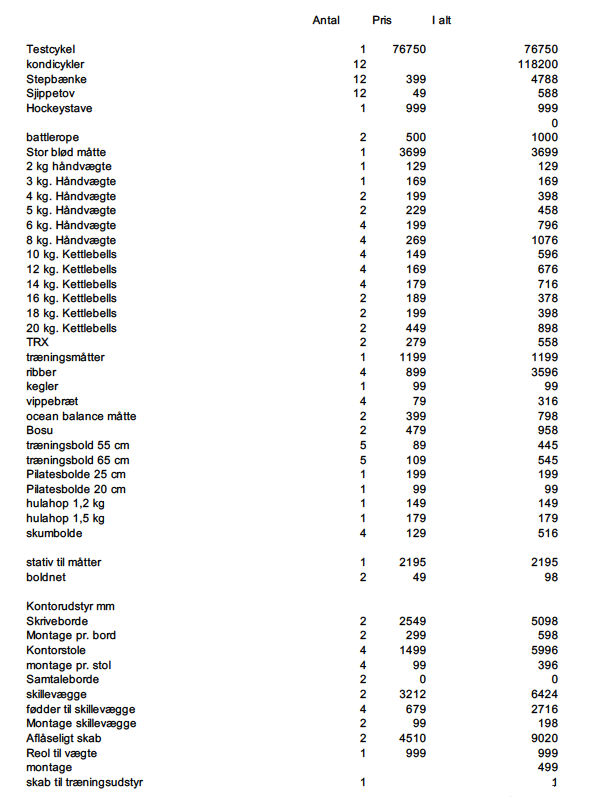
\includegraphics[width=1.0\textwidth]{Figure/8}
\caption{Exercise equipment}

\end{figure} 

 
